\section{事前登録した確認実験}\label{sec:prereg}

\subsection{経緯と登録の内容}

探索段階（G22，CIM 600 ラウンド，seed 0〜255，SA 開始温度 2.0）で，予算 $10^7$ 反転提案（5000 掃引）の SA 後の価値の残差 $r$ と固有ベクトル指標 $E$ の間に順位相関 $\rho=0.57$ が見つかった．指標の定義と使う固有ベクトルの本数はデータを見てから選んだので，定義，解析，判定基準（$\rho$ の 95\% 区間の下限 $>0$）を文書に固定してリポジトリにコミットした後，新しい CIM seed（256〜511）で確かめた．実行は表\ref{tab:prereg}の R1〜R5 の 5 つで，主検定は探索段階と同じ手順の R1 である．候補は $K=256$，SA は各候補 $R=16$ 回で，予算は 50・500・5000 掃引の 3 段階とし，5000 掃引を主予算とした．

\begin{table}[t]
\centering
\caption{事前登録した確認実験の結果（主予算 5000 掃引）．C1 は残差の split-half 信頼性．距離は SA の出力と種のハミング距離の平均（全反転を同一視，頂点数で正規化）．}\label{tab:prereg}
\small
\begin{tabular}{llcccc}
\toprule
実行 & 条件 & $\rho(E, r)$ [95\% 区間] & 判定 & C1 & 距離 \\
\midrule
R1 & G22，600 ラウンド，$T_0=2.0$（主検定） & $0.56$ [$0.46$, $0.65$] & 再現 & $0.89$ & $0.26$ \\
R2 & G22，600 ラウンド，$T_0=4.21$（調整済み） & $-0.02$ [$-0.14$, $0.10$] & 再現せず & $-0.01$ & --- \\
R3 & G22，2400 ラウンド，$T_0=2.0$ & $0.54$ [$0.44$, $0.62$] & 再現 & $0.89$ & $0.26$ \\
R4 & G55，2400 ラウンド，$T_0=2.0$ & $-0.03$ [$-0.15$, $0.10$] & 再現せず & $0.07$ & $0.43$ \\
R5 & G70，2400 ラウンド，$T_0=2.0$ & $0.06$ [$-0.06$, $0.18$] & 再現せず & $0.20$ & $0.44$ \\
\bottomrule
\end{tabular}
\end{table}

\begin{figure}[t]
\centering
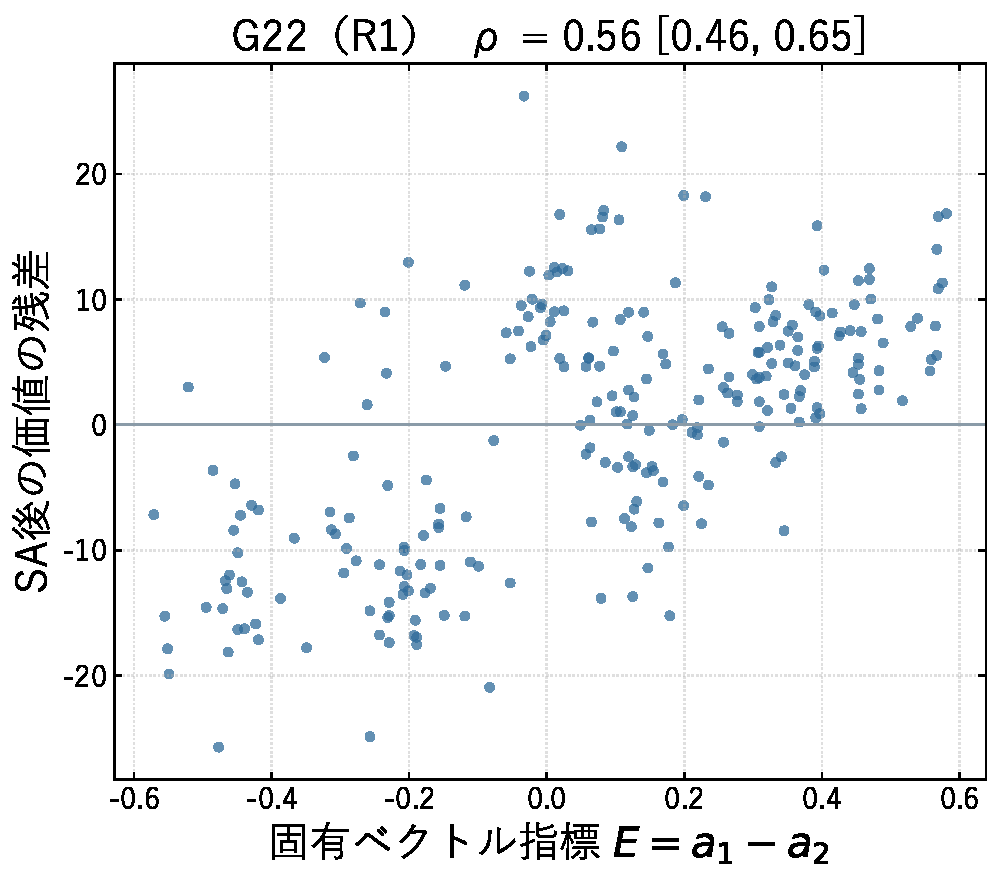
\includegraphics[width=0.42\linewidth]{fig_prereg_scatter.pdf}
\caption{主検定 R1（G22）の候補 256 個．横軸は固有ベクトル指標 $E$，縦軸は SA（5000 掃引）後の価値を初期カット値と LS 後のカット値で回帰した残差．$E$ はいくつかの値の近くに集まり，候補が固有ベクトルの「系統」に分かれることを示す．}\label{fig:prereg_scatter}
\end{figure}

\begin{figure}[t]
\centering
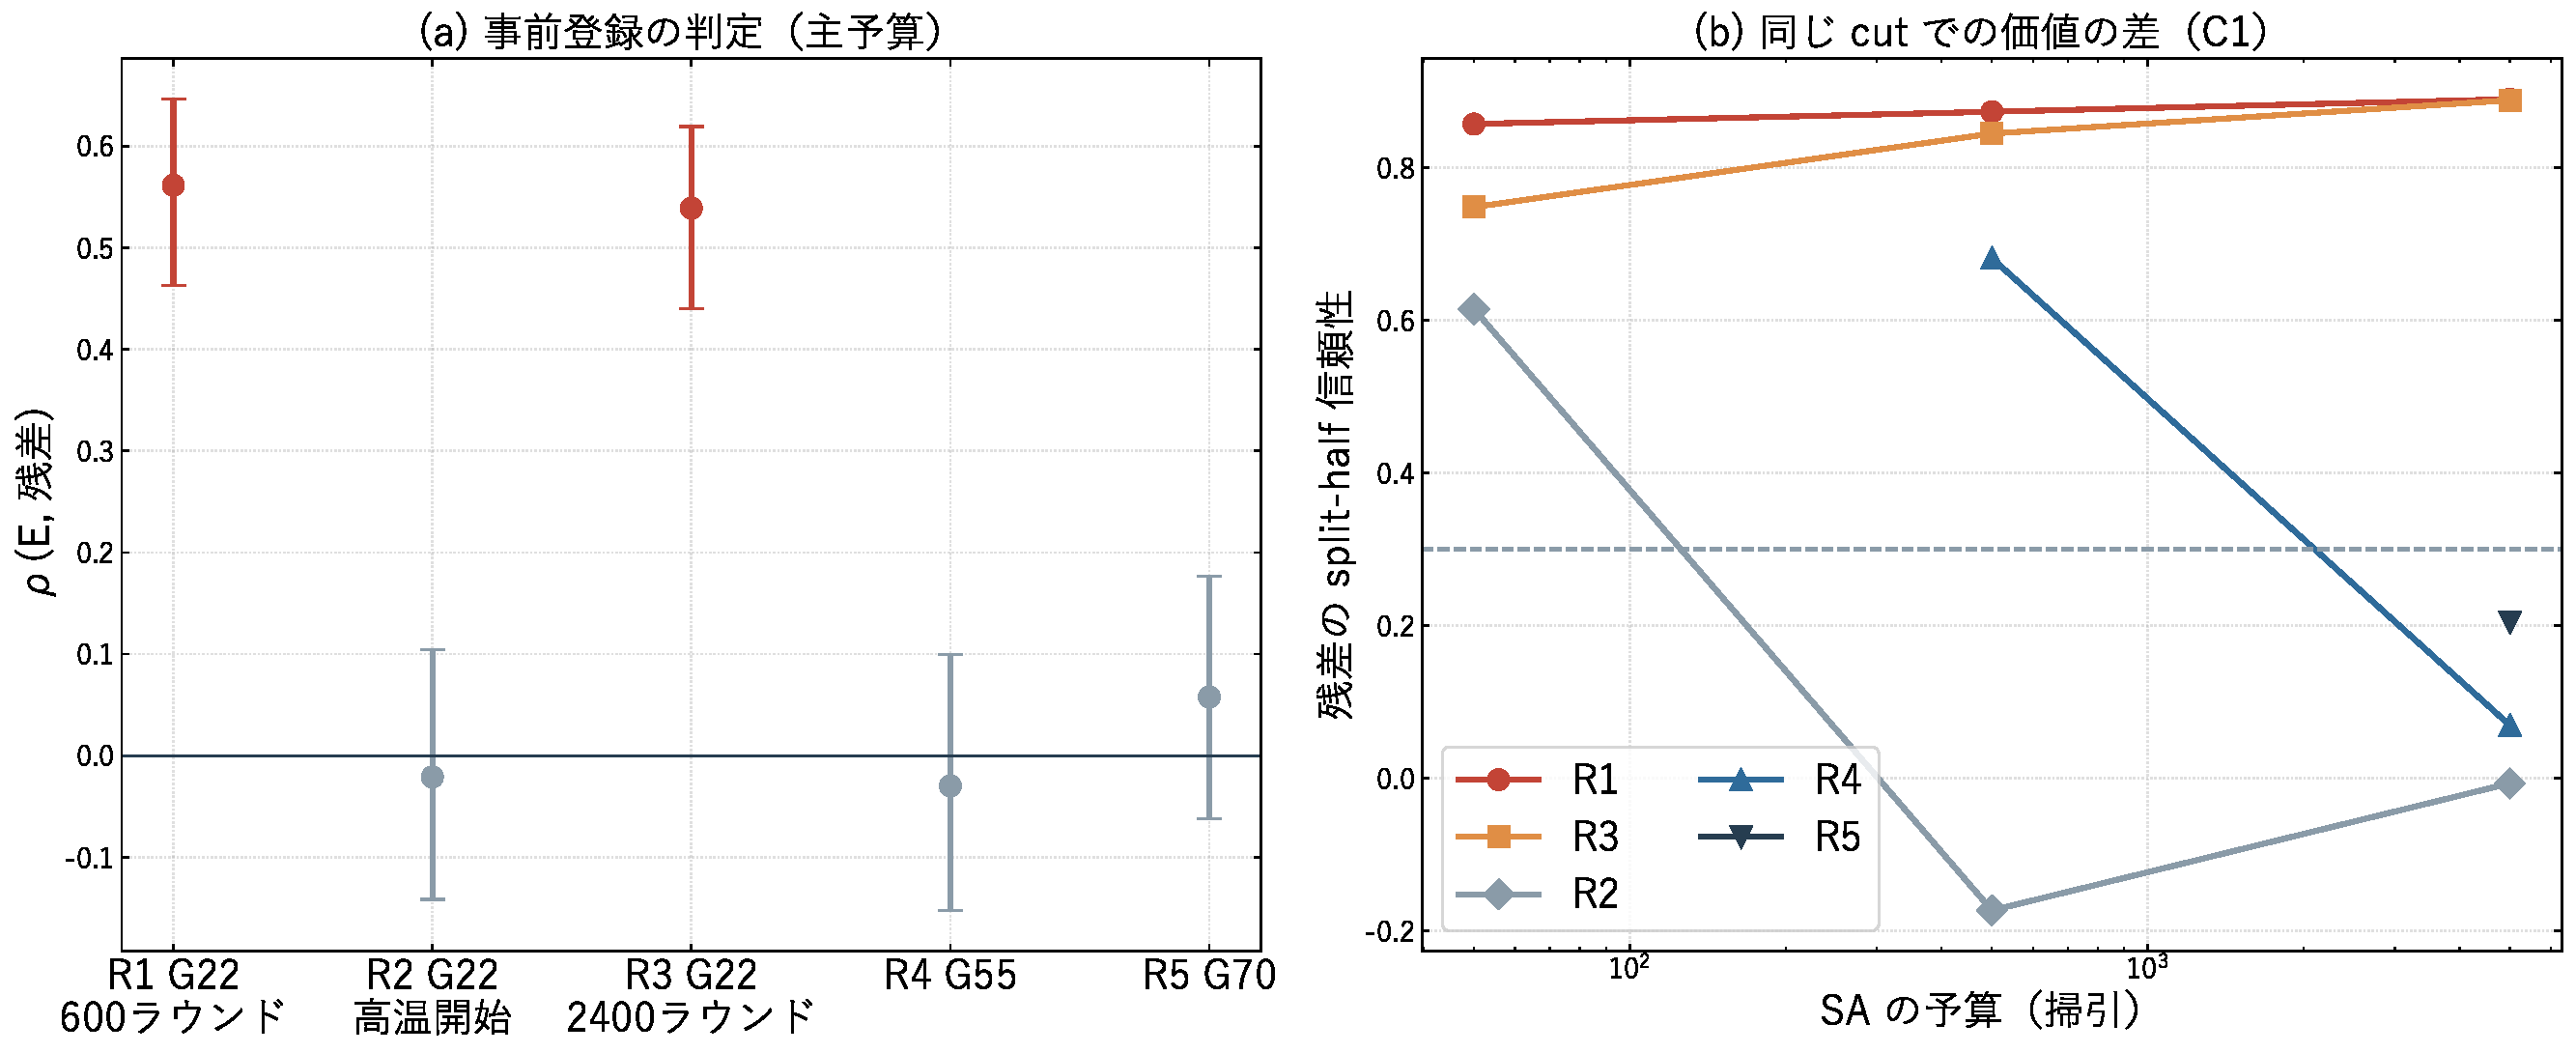
\includegraphics[width=\linewidth]{fig_prereg_summary.pdf}
\caption{(a) 各実行の主予算での $\rho(E, r)$ と 95\% 区間（赤は再現）．(b) 残差の split-half 信頼性（C1）と SA の予算．点線は判定基準 0.3．SA が種を一度も超えずラベルが初期カット値と一致した条件（R4 の 50 掃引，R5 の 50・500 掃引）は判定不能として除いた．}\label{fig:prereg_summary}
\end{figure}

\subsection{結果}

主検定 R1 は再現した（$\rho=0.56$，95\% 区間 [$0.46$, $0.65$]，図\ref{fig:prereg_scatter}）．$E$ は残差の分散の 39\% を説明し，これは SA の乱数で再現できる部分（信頼性 0.89）の 44\% にあたる．CIM を収束まで回した R3 でも同じ大きさで再現した．したがって G22 では，CIM 出力がどちらの固有ベクトルの符号パターンに揃っているかが，カット値と局所探索の改善量では説明できない後段の価値を予測する．

一方，残りの 3 つの実行では再現しなかった．注目すべきは，これらの条件ではそもそも予測すべき差がほとんどなかったことである（図\ref{fig:prereg_summary}(b)）．調整済みの高い開始温度（R2）や，G55・G70 の長い予算（R4・R5）では，SA の出力は種から頂点の 43〜44\% も離れ，残差の信頼性は 0.07〜0.20 に下がった．SA が種をほとんど「忘れる」設定では，同じカット値の候補の価値は等しくなる．G55 の 500 掃引では差が残った（信頼性 0.68）が，$E$ はその差を予測しなかった（$\rho=-0.02$）．

\paragraph{登録後の変更.} warm SA は途中の最良状態（初期解を含む）を返すので，開始温度が高く予算が短いと，SA が一度も種を超えずにラベルが初期カット値と一致する（R4 の 50 掃引，R5 の 50・500 掃引）．このとき残差は恒等的に 0 になり，判定量が定義できない．登録時にはこの場合を想定していなかったので，解析を直してこの場合を判定不能とした．主予算の判定には影響しない．

\paragraph{二峰性について.} 探索段階では，G22 の SA 後の価値が約 13315 と 13345 の 2 群に分かれることを観察していた．同じ判定（GMM の 1 成分と 2 成分の BIC 差 $>10$，Ashman の $D>2$）を当てはめると，ラベルは探索段階・R1・R3 のいずれでも二峰だった．しかし，その由来は一貫しなかった．探索段階では初期カット値が二峰で残差は二峰でなく，R1 では初期カット値は二峰でなく残差が二峰（BIC 差 18.9，$D=3.1$），R3 ではどちらも二峰でなかった．ラベルの二峰性は再現するが，それが初期カット値の分布によるのか，カット値で説明できない部分によるのかは，本論文のデータでは決められない．
